
\newcommand{\depBox}[1]{
	\begin{adjustbox}{minipage=0.90\textwidth,margin=0 \smallskipamount,center}
		Abhängigkeiten:	 #1
	\end{adjustbox} ~\\
}

\section{Module}
\subsection{Modulübersicht}
Die Teilbereiche des Projekts wurden in verschieden Module aufgeteilt.

\begin{figure}[h!]
	\centering
	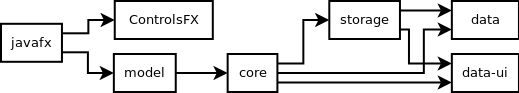
\includegraphics[width=.8\textwidth]{module_dependencies.png}
	\caption{Abhängigkeitsgraph der Module}
	\label{mod_dep_view}
\end{figure}

Der in Abbildung \ref{mod_dep_view} gezeigte Graph enthält keine Abhängigkeiten nach JUnit und
dem JDK aus Gründen der Übersicht.

Anzumerken ist auch, dass bis in das \refLongP{\textModCore} keine Abhängigkeiten
gegenüber einer UI-Bibliothek existieren. Das Modul \hyperref[mod_data-ui]{Data-UI} stellt
zwar Komponenten bereit, die für die Integration in eine Benutzeroberfläche benötigt werden,
bleibt jedoch Benutzeroberflächenunabhängig.


\subsection{\textModCore}
\label{\textModCore}
\begin{figure}[h!]
	\centering
	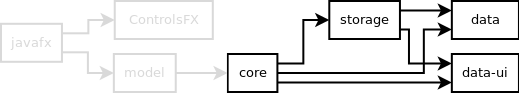
\includegraphics[width=.8\textwidth]{module_dependencies_core.png}
\end{figure}
\depBox{\refLongP{\textModData}, \refLongP{\textModDataUI}, \refLongP{\textModStorage}}

Modulerklräung hier
Core inklusive Abhängigkeiten enthalten alle Logik. Falls eine ander Benutzeroberfläche erstellt,
oder die Logik anderweitig benötigt wird, sollte auf dieses Modul die Abhängigkeit aufgebaut werden.




\subsection{\textModData}
\label{\textModData}
\begin{figure}[h!]
	\centering
	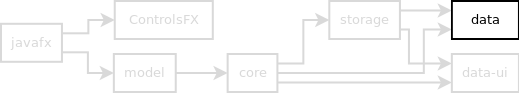
\includegraphics[width=.8\textwidth]{module_dependencies_data.png}
\end{figure}
\depBox{Keine}

Modulerklräung hier




\subsection{\textModDataUI}
\label{\textModDataUI}
\begin{figure}[h!]
	\centering
	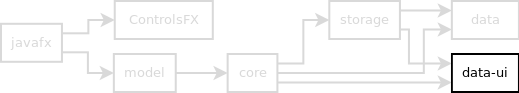
\includegraphics[width=.8\textwidth]{module_dependencies_data-ui.png}
\end{figure}
\depBox{Keine}

Modulerklräung hier




\subsection{\textModJavaFX}
\label{\textModJavaFX}
\begin{figure}[h!]
	\centering
	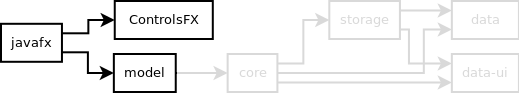
\includegraphics[width=.8\textwidth]{module_dependencies_javafx.png}
\end{figure}
\depBox{\refLongP{\textModModel}, ControlsFX (ext. \cite{controlsfx})}

Modulerklräung hier




\subsection{\textModModel}
\label{\textModModel}
\begin{figure}[h!]
	\centering
	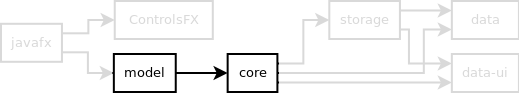
\includegraphics[width=.8\textwidth]{module_dependencies_model.png}
\end{figure}
\depBox{\refLongP{\textModCore}}

Modulerklräung hier




\subsection{\textModStorage}
\label{\textModStorage}
\begin{figure}[h!]
	\centering
	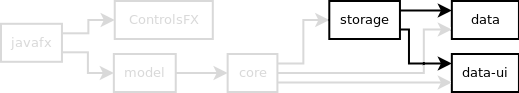
\includegraphics[width=.8\textwidth]{module_dependencies_storage.png}
\end{figure}
\depBox{\refLongP{\textModData}, \refLongP{\textModDataUI}}

Das Storage Modul enthält sowohl eine abstrake Definition von \textit{Serializern} und \textit{StorageHandlern}
als auch eine Implementation für XML inklusive \textit{Serializer} für Komponenten in \refLongP{\textModData} und
\refLongP{\textModDataUI}.

\subsubsection{StorageHandler}
Die Klasse \textit{StorageHandler} ist hält \textit{Storage}s und verteilt Serialisierungsaufgaben an
das entsprechende \textit{Storage} anhand eines Textidentifikators (für XML lautet dieser 'xml').
Eine weitere \textit{Storage} Implementation kann anhand eines neuen Textidentifkators registriert werden,
wodurch ein Umstieg von XML auf JSON, SQL oder eine andere Implementation vereinfacht wird.

\subsubsection{Storage}
Ein \textit{Storage} stellt ein Speicherort für alle zum Projekt gehörenden Komponenten dar. Je nach
Implementation kann dies XML (implementiert), JSON, SQL oder andere sein (nicht implementiert). Bei einem
\textit{Storage} können \textit{Serializer} für weitere Komponenten registriert werden. Sowohl Lese- als
auch Schreibhandles und Hilfsklassen für die \textit{Serializer} werden über Generics in \textit{Storage}
definiert.

\subsubsection{Serializer}
Ein \textit{Serializer} hat die Aufgabe eine Komponente zu serialisieren und wieder zu deserialisieren.
Der Umfang eines \textit{Serializer}s sollte sich auf eine Komponente beziehen (siehe \refLong{\textPrincipleSingleResponsibility}).